\section{Impact of GenAI in the Software Development Process}
\begin{figure}
    \centering
    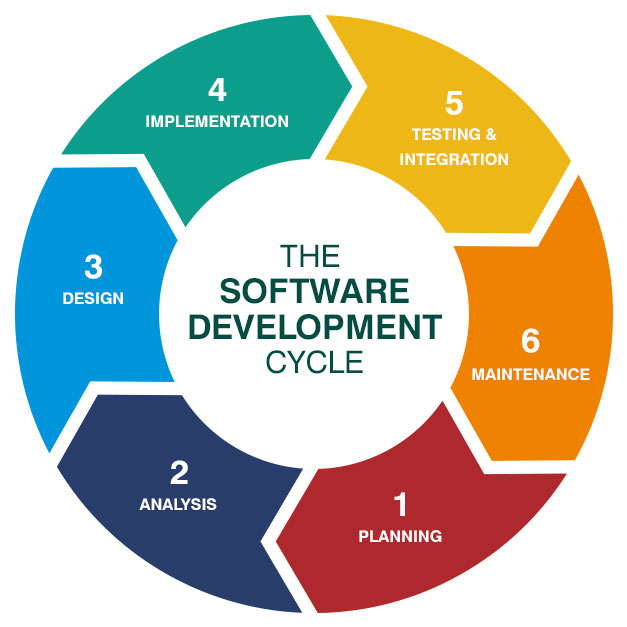
\includegraphics[width=0.75\columnwidth]{content/figures/stages-sdlc.png}
    \caption{The Software Development Life Cycle (SDLC)}
    \label{figure:stages:intro}
\end{figure}
The Software Development Life Cycle (SDLC) (Figure \ref{figure:stages:intro}) is a structured process that guides software development through stages such as requirements elicitation, design, implementation, testing, and deployment. Among these, requirements elicitation is particularly critical, as it involves understanding stakeholder needs and translating them into formal specifications that drive all subsequent stages. This process is inherently human centric and relies heavily on communication, domain expertise, and iterative clarification. However, traditional approaches to requirements engineering often struggle with ambiguity, incomplete information, and the difficulty of training individuals in elicitation skills. In educational settings, this challenge is further compounded by the reliance on static artifacts such as interview transcripts, which allow learners to practice requirement extraction but fail to develop the interactive and exploratory skills required for real-world elicitation scenarios \cite{arora2023advancingrequirements,deniz2022skillsgap}.

The rise of Generative AI, particularly Large Language Models (LLMs), is beginning to transform how SDLC activities—especially requirements engineering—are performed. LLMs like ChatGPT have demonstrated strong capabilities in natural language generation and understanding, enabling them to assist in generating and refining requirements artifacts with high levels of abstraction, consistency, and understandability \cite{aloshan2023zeroshot}. Empirical evidence suggests that AI-generated requirements can match or even outperform human-generated ones across several quality attributes, though challenges such as ambiguity and feasibility remain \cite{bang2023multilingualmultimodalevaluation}. Beyond generation, LLMs can also simulate stakeholders in interactive settings, providing scalable and engaging environments for practicing elicitation skills and improving communication abilities \cite{debnath2020virtualclient}. While these advancements highlight the potential of Generative AI to augment human roles and improve efficiency across the SDLC, they also underscore the continued need for human oversight to ensure correctness, feasibility, and domain alignment.

\begin{table}[t]
    \caption{Software development stages considered in this study}
    \label{tab:stages:re}
    \begin{tabular}{p{0.23\columnwidth} p{0.7\columnwidth}}
        \toprule
        Stage                    & Small description                                                                                                                                                            \\
        \midrule
        Requirements Elicitation & Gathering, clarifying, and structuring user needs and system expectations; involves understanding ambiguity, stakeholder communication, and defining what needs to be built. \\

        Coding                   & Translating requirements into executable code; includes implementation, API usage, logic construction, and integration of components.                                        \\

        Debugging                & Identifying, analyzing, and fixing errors or unintended behavior in code; involves reasoning about program execution and validating correctness.                             \\

        Documentation            & Creating explanations, comments, and supporting material for code and systems; helps with knowledge transfer, maintainability, and onboarding.                               \\
        \bottomrule
    \end{tabular}
\end{table}

For the purposes of this paper, we focus on four key stages of the SDLC that are particularly impacted by Generative AI: requirements elicitation, coding, debugging, and documentation (Table \ref{tab:stages:re}). These stages represent critical points in the development process where human-AI interaction can significantly influence developer behavior, problem-solving strategies, and overall productivity.